\documentclass[aspectratio=169,10pt]{beamer}

% Theme selection
\usetheme{AnnArbor}
\usecolortheme{dolphin}

% Font and encoding
\usepackage{fontspec}
\setmainfont{DejaVu Sans}
\setsansfont{DejaVu Sans}
\setmonofont{Consolas}

\usepackage{booktabs}
\usepackage{array}
\usepackage{tabularx}
\usepackage{listings}
\usepackage{tikz}
\usepackage{amsmath}
\usepackage{amssymb}
\usepackage{adjustbox}
\usetikzlibrary{shapes,arrows,positioning,calc}

% Color definitions
\definecolor{codegray}{rgb}{0.95,0.95,0.95}
\definecolor{codeblue}{rgb}{0.1,0.2,0.6}
\definecolor{codegreen}{rgb}{0.1,0.5,0.1}
\definecolor{crimsonred}{rgb}{0.8,0.1,0.1}
\definecolor{darkgreen}{rgb}{0.0,0.4,0.0}
\definecolor{accentorange}{rgb}{0.85,0.4,0.0}

% Custom code style
\newcommand{\code}[1]{\texttt{\textcolor{codeblue}{#1}}}

% Slide Metadata
\title[Clustering in Machine Learning]{\Large \textbf{CLUSTERING IN MACHINE LEARNING}}
\subtitle{\normalsize Comprehensive Theory, Formula Intuition, Hand Calculations, Real-World Applications \& Decision Guide}
\author[Dr. Minh Duc Vu]{Dr. Minh Duc Vu}
\institute[NEU]{Department of Data Science and Artificial Intelligence\\College of Technology -- National Economics University (NEU)}
\date{2026}

\begin{document}

% Slide 1: Title
\begin{frame}
  \titlepage
\end{frame}

% Slide 2: Learning Objectives
\begin{frame}{Learning Objectives}
  \small
  \begin{itemize}\setlength{\itemsep}{2.5pt}
    \item \textbf{Essence of Clustering:} Master the philosophy of Unsupervised Learning and clearly distinguish between \textbf{Hard Clustering} and \textbf{Soft Clustering}.
    \item \textbf{Formula Intuition \& Distance Metrics:} Understand the mathematical rationale behind WCSS, Linkage criteria, $\varepsilon$-neighborhood density, Bayes' rule in EM, and Silhouette analysis.
    \item \textbf{Master 5 Core Clustering Paradigms via Step-by-Step Hand Calculations:}
      \begin{enumerate}\setlength{\itemsep}{1.5pt}
        \item \textbf{Centroid-based:} K-Means, K-Means++, Elbow Method, K-Medoids.
        \item \textbf{Connectivity-based:} Hierarchical Clustering, Dendrogram, 5 Linkage Criteria.
        \item \textbf{Density-based:} DBSCAN (Core/Border/Noise), OPTICS (Reachability Plot).
        \item \textbf{Distribution-based:} Gaussian Mixture Models (GMM), Expectation-Maximization (EM).
        \item \textbf{Fuzzy Clustering:} Fuzzy C-Means (FCM) with membership degree $u_{ik}$.
      \end{enumerate}
    \item \textbf{Breakthrough Real-World Applications:} Examine high-impact use cases across E-commerce, Bioinformatics, Fraud Detection, GPS Fleet Telematics, and Speech Processing.
    \item \textbf{Model Selection Guide:} Master the practical decision tree and scenario suitability matrix to select the optimal clustering model for production environments.
  \end{itemize}
\end{frame}

% Slide 3: Overview of Unsupervised Learning & Clustering
\begin{frame}{1. The Essence of Data Clustering}
  \begin{columns}[T]
    \begin{column}{0.55\textwidth}
      \textbf{Foundational Concept:}
      \begin{itemize}\setlength{\itemsep}{2pt}
        \item The central problem in \textbf{Unsupervised Machine Learning}.
        \item Input data consists solely of feature vectors $\mathcal{X} = \{x_1, \dots, x_N\}$, with \textbf{no ground truth target labels} $y$.
        \item \textbf{Primary Objective:} Automatically group observations into clusters such that:
          \begin{itemize}\setlength{\itemsep}{1pt}
            \item \textbf{High Intra-cluster Similarity:} Points within the same cluster are as close/similar as possible.
            \item \textbf{High Inter-cluster Dissimilarity:} Points in different clusters are as distant/distinct as possible.
          \end{itemize}
        \item A cluster is an intrinsic grouping defined by proximity, density, or distribution geometry.
      \end{itemize}
    \end{column}
    \begin{column}{0.45\textwidth}
      \begin{center}
        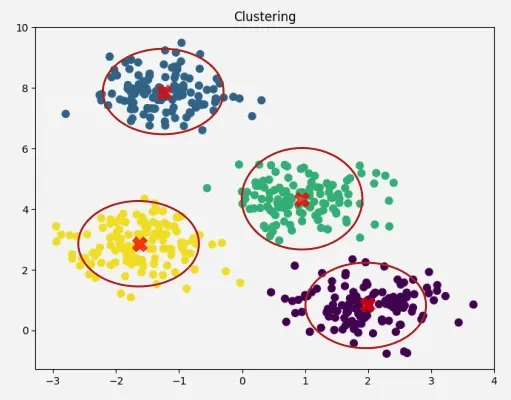
\includegraphics[width=0.95\linewidth,height=0.65\textheight,keepaspectratio]{images/clustering-overview.png}
      \end{center}
    \end{column}
  \end{columns}
\end{frame}

% Slide 4: Hard vs Soft Clustering
\begin{frame}{Taxonomy by Assignment: Hard vs Soft Clustering}
  \begin{columns}[T]
    \begin{column}{0.52\textwidth}
      \textbf{1. Hard Clustering (Exclusive Assignment):}
      \begin{itemize}\setlength{\itemsep}{2pt}
        \item Each data point $x_i$ is assigned strictly to a single cluster $C_k$ ($100\%$ membership).
        \item Binary membership indicator: $z_{ik} \in \{0, 1\}$ satisfying $\sum_{k=1}^K z_{ik} = 1$.
        \item \textit{Archetypes:} K-Means, Hierarchical Clustering, DBSCAN.
      \end{itemize}
      \vspace{0.4em}
      \textbf{2. Soft / Fuzzy Clustering (Probabilistic Assignment):}
      \begin{itemize}\setlength{\itemsep}{2pt}
        \item Each point belongs to all clusters simultaneously via \textbf{posterior probabilities} or fuzzy degrees $\gamma_{ik} \in [0, 1]$ satisfying $\sum_{k=1}^K \gamma_{ik} = 1$.
        \item \textit{Archetypes:} Gaussian Mixture Models (EM), Fuzzy C-Means (FCM).
      \end{itemize}
    \end{column}
    \begin{column}{0.48\textwidth}
      \begin{center}
        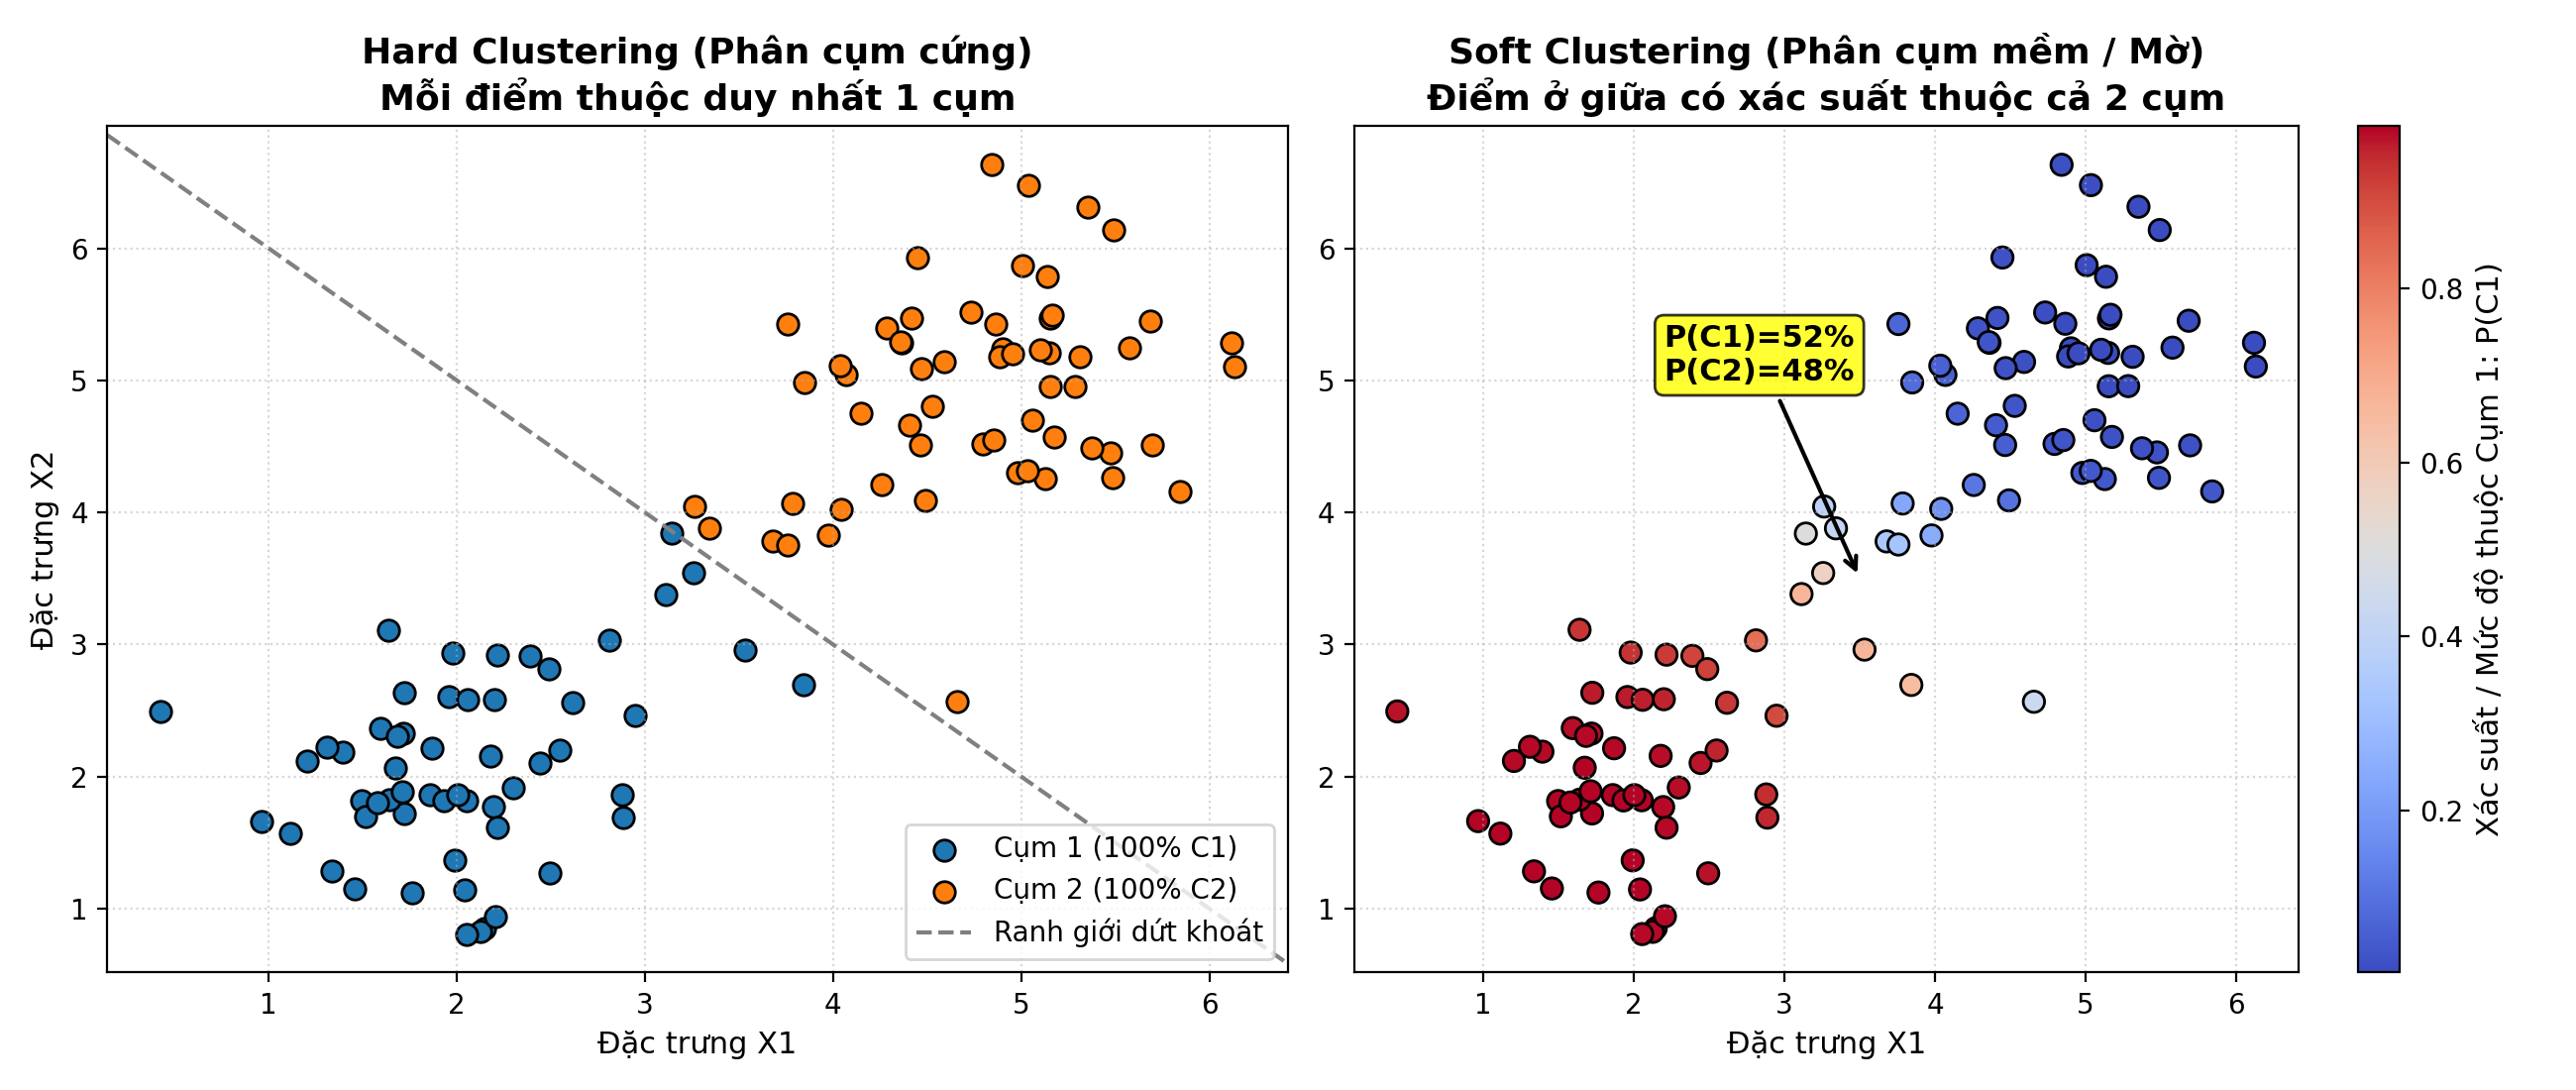
\includegraphics[width=0.98\linewidth,height=0.65\textheight,keepaspectratio]{images/hard-vs-soft-clustering.png}
      \end{center}
    \end{column}
  \end{columns}
\end{frame}

% Slide 5: Distance Metrics & Normalization
\begin{frame}{Distance Metrics \& The Vital Role of Feature Scaling}
  \small
  \begin{columns}[T]
    \begin{column}{0.52\textwidth}
      \textbf{Common Metric Formulations:}
      \begin{itemize}\setlength{\itemsep}{2pt}
        \item \textbf{Euclidean Distance ($L_2$ norm):}
          $$d(x, z) = \sqrt{\sum_{j=1}^d (x_j - z_j)^2}$$
          Gold standard for continuous, isotropic quantitative variables.
        \item \textbf{Manhattan Distance ($L_1$ norm / City Block):}
          $$d(x, z) = \sum_{j=1}^d |x_j - z_j|$$
          More robust to outliers, natural in grid-like feature spaces.
        \item \textbf{Cosine Similarity (Angular metric):}
          $$\cos(\theta) = \frac{x \cdot z}{\|x\|_2 \|z\|_2}$$
          Standard for high-dimensional text (TF-IDF) and embeddings.
      \end{itemize}
    \end{column}
    \begin{column}{0.48\textwidth}
      \begin{center}
        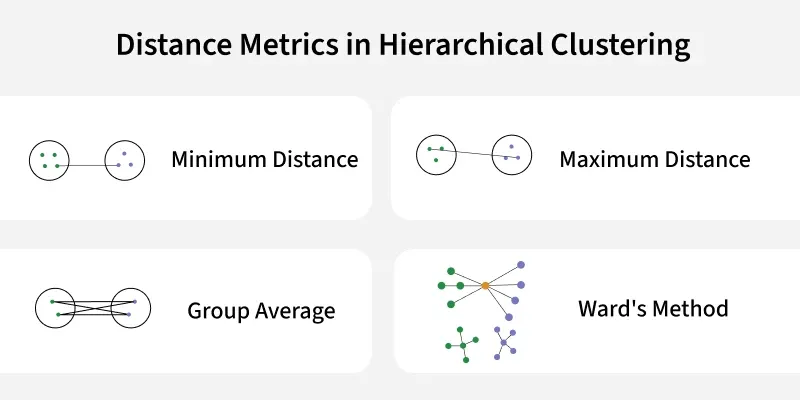
\includegraphics[width=0.98\linewidth,height=0.38\textheight,keepaspectratio]{images/distance-metrics.png}
      \end{center}
      \footnotesize
      \textbf{Vital Caveat:} Always perform \textbf{Feature Scaling (\code{StandardScaler})} before computing distances! Unscaled features with large ranges (e.g., Annual Income $\$10^5$) will completely dominate smaller features (e.g., Age $10^1$).
    \end{column}
  \end{columns}
\end{frame}

% Slide 6: Big Picture - 5 Paradigms
\begin{frame}{The Big Picture: 5 Major Clustering Paradigms}
  \begin{table}[]
    \scriptsize
    \centering
    \begin{tabularx}{\textwidth}{l p{2.6cm} p{2.6cm} X}
      \toprule
      \textbf{Paradigm} & \textbf{Core Philosophy} & \textbf{Key Algorithms} & \textbf{Geometric Properties} \\
      \midrule
      \textbf{Centroid-based} & Represents each cluster by a central prototype & K-Means, K-Means++, K-Medoids & Convex, spherical clusters (Voronoi cells) \\
      \addlinespace
      \textbf{Connectivity} & Groups samples based on proximity hierarchy & Agglomerative, Divisive, BIRCH & Multi-level tree structure (Dendrogram) \\
      \addlinespace
      \textbf{Density-based} & Clusters are dense regions separated by low-density zones & DBSCAN, OPTICS, HDBSCAN & Arbitrary non-linear shapes; automated noise filter \\
      \addlinespace
      \textbf{Distribution} & Assumes data is generated from a mixture of distributions & Gaussian Mixture Models (GMM), EM & Flexible oriented ellipsoids; soft membership \\
      \addlinespace
      \textbf{Fuzzy / Soft} & Points belong to clusters with continuous fuzzy degrees & Fuzzy C-Means (FCM) & Overlapping clusters; gradual boundary transitions \\
      \bottomrule
    \end{tabularx}
  \end{table}
\end{frame}

% Slide 7: Centroid-based - K-Means
\begin{frame}{2. Centroid-based: Classical K-Means Algorithm}
  \small
  \begin{columns}[T]
    \begin{column}{0.55\textwidth}
      \textbf{Lloyd's 4-Step Heuristic (1957):}
      \begin{enumerate}\setlength{\itemsep}{1pt}
        \item \textbf{Initialization:} Choose $K$ initial cluster centroids $\mu_1, \dots, \mu_K$.
        \item \textbf{Assignment Step:} Assign each data point $x_i$ to the nearest centroid:
          $$c^{(i)} = \arg\min_k \|x_i - \mu_k\|_2^2$$
        \item \textbf{Update Step:} Recalculate centroids as the arithmetic mean of assigned points:
          $$\mu_k = \frac{1}{|C_k|} \sum_{x_i \in C_k} x_i$$
        \item \textbf{Iterate} Steps 2 and 3 until centroids converge (no reassignments).
      \end{enumerate}
      \textbf{Objective Function (WCSS / Inertia):}
      $$J = \sum_{k=1}^K \sum_{x_i \in C_k} \|x_i - \mu_k\|_2^2 \to \min$$
    \end{column}
    \begin{column}{0.45\textwidth}
      \begin{center}
        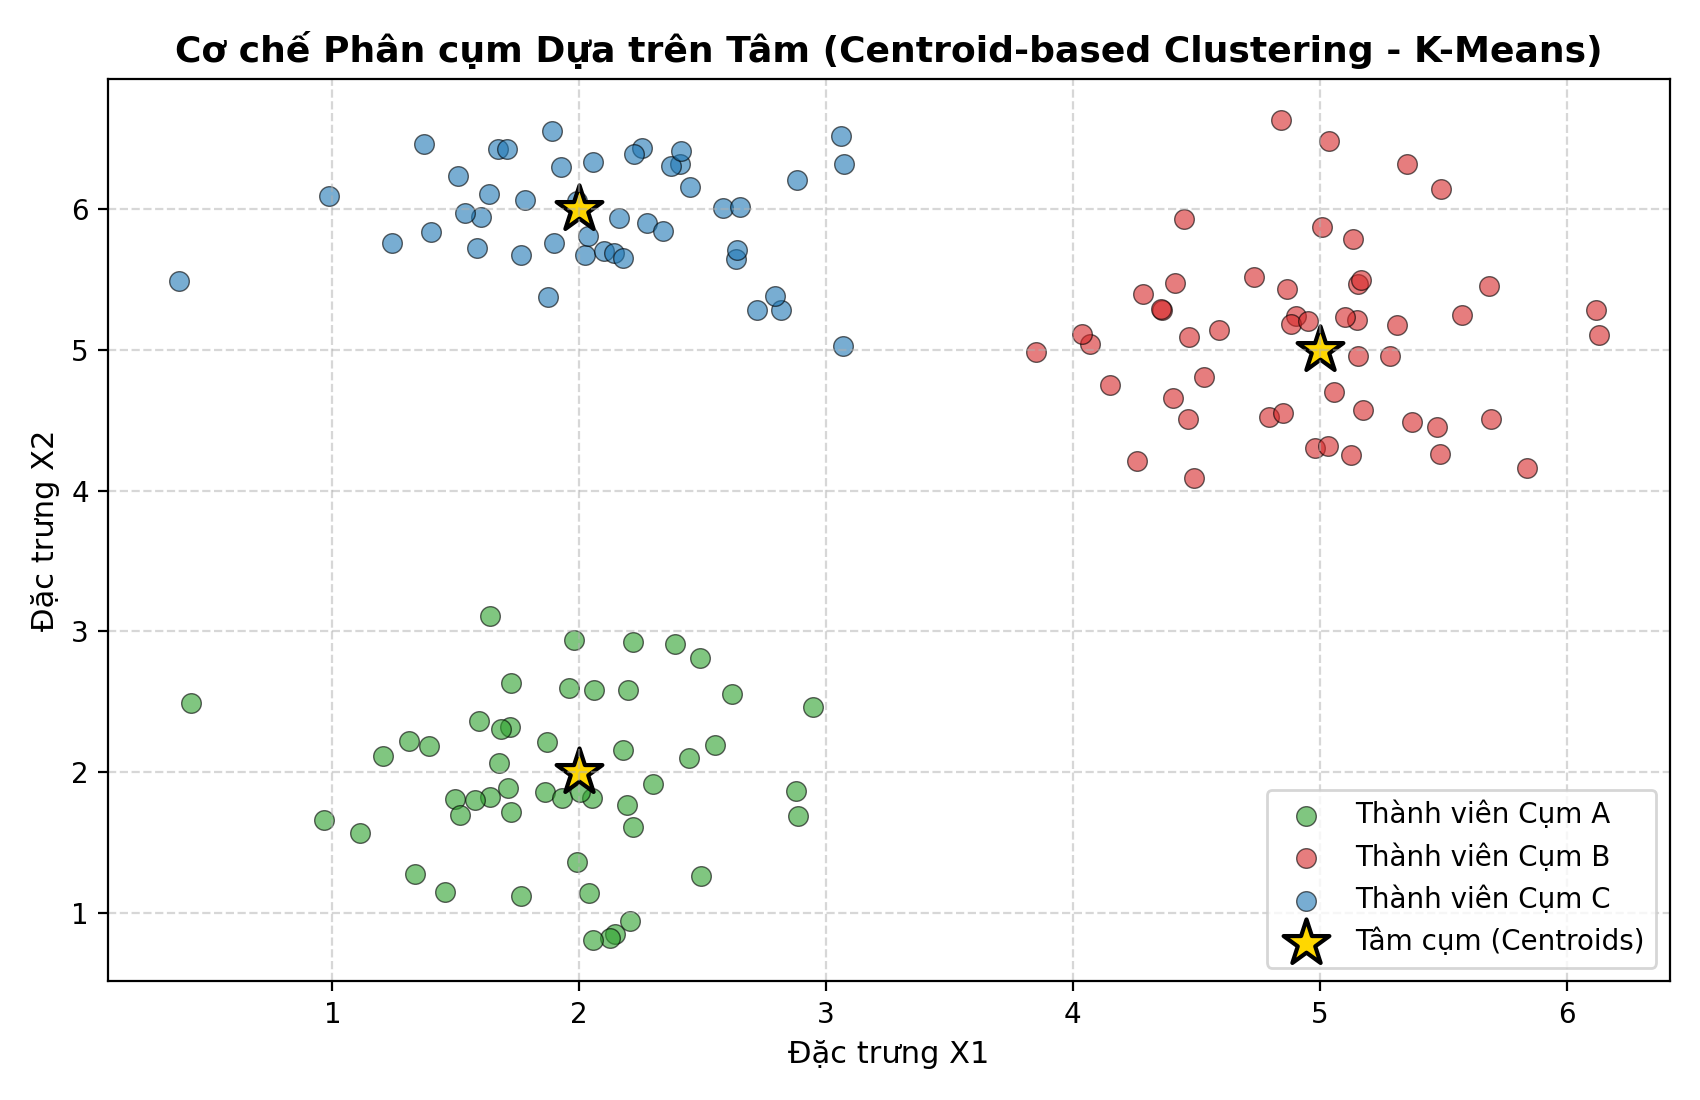
\includegraphics[width=0.95\linewidth,height=0.62\textheight,keepaspectratio]{images/centroid-based-kmeans.png}
      \end{center}
    \end{column}
  \end{columns}
\end{frame}

% Slide 8: K-Means - Formula Intuition
\begin{frame}{K-Means: Mathematical Rationale \& Formula Intuition}
  \footnotesize
  \begin{columns}[T]
    \begin{column}{0.5\textwidth}
      \textbf{1. Intuition of the WCSS Objective (Inertia):}
      $$J = \sum_{k=1}^K \sum_{x_i \in C_k} \|x_i - \mu_k\|_2^2$$
      \begin{itemize}\setlength{\itemsep}{1.5pt}
        \item Measures the \textbf{total squared deviation} of points from their respective cluster prototypes.
        \item Minimizing $J$ directly minimizes the total intra-cluster sample variance (cluster compactness).
        \item \textbf{Why the arithmetic mean?} Taking partial derivatives with respect to $\mu_k$:
          $$\frac{\partial J}{\partial \mu_k} = -2\sum_{x_i \in C_k} (x_i - \mu_k) = 0 \implies \mu_k = \frac{1}{|C_k|}\sum_{x_i \in C_k} x_i$$
          $\to$ The mean is the unique closed-form minimizer for squared Euclidean distance!
      \end{itemize}
    \end{column}
    \begin{column}{0.5\textwidth}
      \textbf{2. Intuition of K-Means++ Initialization:}
      $$P(x) = \frac{D(x)^2}{\sum_{x' \in \mathcal{X}} D(x')^2}$$
      \begin{itemize}\setlength{\itemsep}{1.5pt}
        \item $D(x)$: Shortest distance from candidate $x$ to any already chosen centroid.
        \item \textbf{Intuition:} The squared distance $D(x)^2$ heavily penalizes choosing candidates close to existing centroids.
        \item \textbf{Vital Effect:} Forcibly disperses initial centroids across the entire feature space, avoiding redundant centroids in dense regions.
        \item \textbf{Theoretical Guarantee:} Reduces worst-case $O(e^K)$ local-minima risk to an expected $O(\log K)$-competitive bound against the global optimum.
      \end{itemize}
    \end{column}
  \end{columns}
\end{frame}

% Slide 9: Hand Calculation K-Means
\begin{frame}{K-Means: Step-by-Step Hand Calculation (1 Iteration)}
  \scriptsize
  \textbf{Sample Problem:} Consider 4 points in $\mathbb{R}^2$: $A(1, 1), B(2, 1), C(4, 3), D(5, 4)$. Cluster into $K=2$ groups.\\
  \textbf{Initialization:} Seed initial centroids at $\mu_1^{(0)} = A(1, 1)$ and $\mu_2^{(0)} = D(5, 4)$.
  
  \vspace{0.4em}
  \begin{columns}[T]
    \begin{column}{0.5\textwidth}
      \textbf{Step 1: Compute Squared Distances \& Assign}
      \begin{itemize}\setlength{\itemsep}{1pt}
        \item Point $A(1, 1)$:
          $d^2(A, \mu_1) = 0$; $d^2(A, \mu_2) = (1-5)^2 + (1-4)^2 = 16 + 9 = \mathbf{25} \implies \mathbf{A \in C_1}$.
        \item Point $B(2, 1)$:
          $d^2(B, \mu_1) = (2-1)^2 + 0 = \mathbf{1}$; $d^2(B, \mu_2) = 9 + 9 = 18 \implies \mathbf{B \in C_1}$.
        \item Point $C(4, 3)$:
          $d^2(C, \mu_1) = 9 + 4 = 13$; $d^2(C, \mu_2) = (4-5)^2 + (3-4)^2 = \mathbf{2} \implies \mathbf{C \in C_2}$.
        \item Point $D(5, 4)$:
          $d^2(D, \mu_1) = 16 + 9 = 25$; $d^2(D, \mu_2) = \mathbf{0} \implies \mathbf{D \in C_2}$.
      \end{itemize}
      $\implies$ Iteration 1 Partition: $C_1 = \{A, B\}$, $C_2 = \{C, D\}$.
    \end{column}
    \begin{column}{0.5\textwidth}
      \textbf{Step 2: Update Centroid Coordinates $\mu^{(1)}$}
      $$\mu_1^{(1)} = \frac{A + B}{2} = \left(\frac{1+2}{2}, \frac{1+1}{2}\right) = \mathbf{(1.5, 1.0)}$$
      $$\mu_2^{(1)} = \frac{C + D}{2} = \left(\frac{4+5}{2}, \frac{3+4}{2}\right) = \mathbf{(4.5, 3.5)}$$
      \vspace{0.2em}
      \textbf{Step 3: Evaluate WCSS ($J$) Reduction}
      \begin{itemize}\setlength{\itemsep}{1pt}
        \item $J^{(0)} = d^2(A, \mu_1^{(0)}) + d^2(B, \mu_1^{(0)}) + d^2(C, \mu_2^{(0)}) + d^2(D, \mu_2^{(0)}) = 0 + 1 + 2 + 0 = \mathbf{3.0}$.
        \item $J^{(1)} = 2 \times [(0.5)^2 + 0] + 2 \times [(0.5)^2 + (0.5)^2] = 0.5 + 1.0 = \mathbf{1.5}$.
      \end{itemize}
      $\implies$ WCSS drops from $3.0 \to 1.5$! Next iteration produces identical assignments $\to$ Converged!
    \end{column}
  \end{columns}
\end{frame}

% Slide 10: Centroid-based - Applications & Suitability
\begin{frame}{Centroid-based: Real-World Applications \& Suitability Guide}
  \small
  \begin{columns}[T]
    \begin{column}{0.5\textwidth}
      \textbf{1. Practical Applications:}
      \begin{itemize}\setlength{\itemsep}{2pt}
        \item \textbf{RFM Customer Segmentation (E-commerce):}
          E-commerce platforms (Amazon, Shopee) segment millions of customers along Recency, Frequency, and Monetary dimensions into $K=4$ actionable tiers: VIP Champions, Loyal Core, Promising, and Churn Risk.
        \item \textbf{Color Quantization / Image Compression:}
          24-bit RGB images contain up to $16.7$M colors. K-Means clusters pixel vectors into $K=16$ or $64$ centroid palette colors, saving $75-85\%$ file size with minimal perceptual degradation.
        \item \textbf{Supply Chain Hub Location:}
          Optimizes warehouse and EV fast-charging coordinates by minimizing aggregate transport distance.
      \end{itemize}
    \end{column}
    \begin{column}{0.5\textwidth}
      \textbf{2. When to Use vs When NOT to Use:}
      \begin{itemize}\setlength{\itemsep}{2pt}
        \item \textcolor{darkgreen}{\textbf{RECOMMENDED WHEN:}}
          \begin{itemize}
            \item Large-scale tabular datasets ($N > 10^5 \to 10^7$).
            \item Clusters are predominantly convex, spherical, and of comparable scale and variance.
            \item High inference speed and simple production explainability are mandatory.
          \end{itemize}
        \item \textcolor{crimsonred}{\textbf{AVOID WHEN:}}
          \begin{itemize}
            \item Clusters have non-convex geometries (crescents, rings, spirals).
            \item Heavy outlier contamination (switch to \textbf{K-Medoids / PAM}).
            \item Highly disparate cluster densities.
          \end{itemize}
      \end{itemize}
    \end{column}
  \end{columns}
\end{frame}

% Slide 11: Connectivity-based - Hierarchical
\begin{frame}{3. Connectivity-based: Hierarchical Clustering}
  \begin{columns}[T]
    \begin{column}{0.55\textwidth}
      \textbf{Two Dual Methodologies:}
      \begin{enumerate}\setlength{\itemsep}{2pt}
        \item \textbf{Agglomerative (Bottom-Up):}
          \begin{itemize}
            \item Starts with $N$ singleton clusters (leaves).
            \item Sequentially merges the two closest clusters.
            \item Terminates at a single root cluster.
          \end{itemize}
        \item \textbf{Divisive (Top-Down):}
          \begin{itemize}
            \item Starts with 1 comprehensive cluster.
            \item Recursively splits clusters into finer sub-groups.
          \end{itemize}
      \end{enumerate}
      \textbf{Key Advantage:} Does not require pre-specifying the number of clusters $K$ beforehand! Exposes multi-scale taxonomy.
    \end{column}
    \begin{column}{0.45\textwidth}
      \begin{center}
        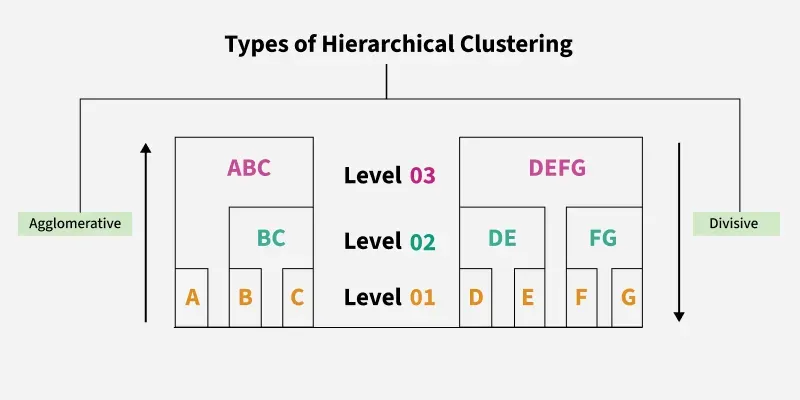
\includegraphics[width=0.95\linewidth,height=0.62\textheight,keepaspectratio]{images/types-of-hierarchical-clustering.png}
      \end{center}
    \end{column}
  \end{columns}
\end{frame}

% Slide 12: Hierarchical - Formula Intuition
\begin{frame}{Hierarchical: Mathematical Rationale \& 5 Linkage Criteria}
  \footnotesize
  \begin{columns}[T]
    \begin{column}{0.5\textwidth}
      \textbf{1. Single Linkage (Minimum Distance):}
      $$D(A, B) = \min_{x \in A, y \in B} d(x, y)$$
      \begin{itemize}\setlength{\itemsep}{1pt}
        \item \textbf{Intuition:} Merges clusters based on the shortest inter-cluster point pair (nearest-neighbor connectivity).
        \item \textbf{Fatal Flaw:} Vulnerable to the \textbf{Chaining Effect} -- a sparse bridge of noise points can artificially chain two large, distinct clusters together.
      \end{itemize}
      \vspace{0.2em}
      \textbf{2. Complete Linkage (Maximum Distance):}
      $$D(A, B) = \max_{x \in A, y \in B} d(x, y)$$
      \begin{itemize}\setlength{\itemsep}{1pt}
        \item \textbf{Intuition:} Based on the maximum pairwise diameter. Forces compact, tight spherical clusters; highly sensitive to outliers.
      \end{itemize}
    \end{column}
    \begin{column}{0.5\textwidth}
      \textbf{3. Average Linkage (Mean Proximity):}
      $$D(A, B) = \frac{1}{|A||B|}\sum_{x \in A}\sum_{y \in B} d(x, y)$$
      \begin{itemize}\setlength{\itemsep}{1pt}
        \item Balanced compromise between Single and Complete; robust to moderate noise.
      \end{itemize}
      \vspace{0.2em}
      \textbf{4. Ward's Minimum Variance Method:}
      $$\Delta \text{WCSS} = \frac{|A||B|}{|A| + |B|}\|\mu_A - \mu_B\|_2^2$$
      \begin{itemize}\setlength{\itemsep}{1pt}
        \item \textbf{Intuition:} Merges the pair that produces the \textbf{smallest increase in total within-cluster variance}.
        \item \textbf{Empirical Recommendation:} \textbf{Most effective and widely used} linkage criterion on real-world datasets!
      \end{itemize}
    \end{column}
  \end{columns}
\end{frame}

% Slide 13: Hand Calculation Hierarchical
\begin{frame}{Hierarchical: Step-by-Step Hand Calculation \& Dendrogram}
  \scriptsize
  \textbf{Sample Problem:} Consider 3 points in 1D: $A=1.0, B=2.0, C=6.0$. Perform Agglomerative Hierarchical Clustering.\\
  \textbf{Initial Distance Matrix $D_0$:} $d(A, B) = |1-2| = \mathbf{1.0}$, $d(B, C) = |2-6| = \mathbf{4.0}$, $d(A, C) = |1-6| = \mathbf{5.0}$.
  
  \vspace{0.4em}
  \begin{columns}[T]
    \begin{column}{0.5\textwidth}
      \textbf{Step 1: Merge the Closest Pair}
      \begin{itemize}\setlength{\itemsep}{1.5pt}
        \item The minimum entry is $(A, B)$ with $d(A, B) = \mathbf{1.0}$.
        \item Merge into new cluster $C_1 = \{A, B\}$ at merge height $h = 1.0$.
      \end{itemize}
      \vspace{0.2em}
      \textbf{Step 2: Update Proximity from $\{A, B\}$ to $C$}
      \begin{itemize}\setlength{\itemsep}{1.5pt}
        \item \textbf{Single Linkage:}
          $$D_{\text{single}} = \min(d_{AC}, d_{BC}) = \min(5, 4) = \mathbf{4.0}$$
        \item \textbf{Complete Linkage:}
          $$D_{\text{complete}} = \max(d_{AC}, d_{BC}) = \max(5, 4) = \mathbf{5.0}$$
        \item \textbf{Ward's Method ($\mu_{\{A,B\}} = 1.5, \mu_C = 6$):}
          $$\Delta \text{WCSS} = \frac{2 \times 1}{2 + 1}(1.5 - 6)^2 = \frac{2}{3} \times 20.25 = \mathbf{13.5}$$
      \end{itemize}
    \end{column}
    \begin{column}{0.5\textwidth}
      \textbf{Step 3: Dendrogram Cutting Analysis}
      \begin{center}
        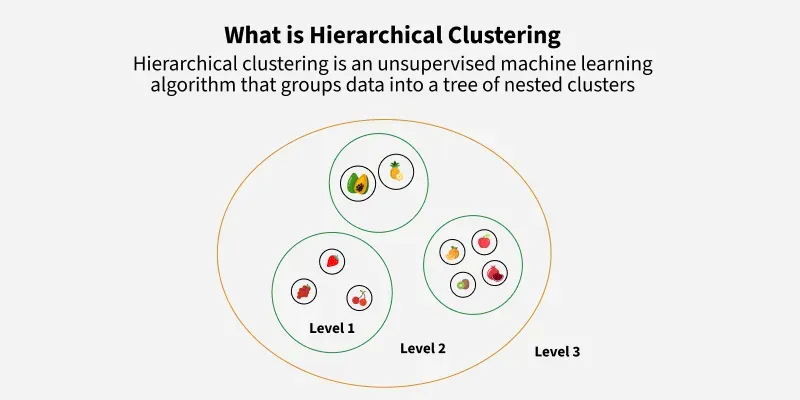
\includegraphics[width=0.92\linewidth,height=0.36\textheight,keepaspectratio]{images/longest-path-dendrogram.png}
      \end{center}
      \textbf{Optimal Cutting Rule:}
      \begin{itemize}\setlength{\itemsep}{1pt}
        \item To obtain $K=2$ clusters: Cut across height $1.5 < h < 4.0$. Resulting clusters: $\{A, B\}$ and $\{C\}$.
        \item The vertical gap from $1.0 \to 4.0$ (span $\Delta h = 3.0$) is the longest uninterrupted vertical branch $\to$ Confirms $K=2$ is the most salient natural structure!
      \end{itemize}
    \end{column}
  \end{columns}
\end{frame}

% Slide 14: Connectivity-based - Applications & Suitability
\begin{frame}{Connectivity-based: Real-World Applications \& Suitability Guide}
  \footnotesize
  \begin{columns}[T]
    \begin{column}{0.5\textwidth}
      \textbf{1. Practical Applications:}
      \begin{itemize}\setlength{\itemsep}{2pt}
        \item \textbf{Bioinformatics \& Gene Expression (Clustered Heatmap):}
          Hierarchical clustering groups thousands of gene microarray/RNA-seq profiles simultaneously across patient samples, discovering co-expressed oncogene pathways and drug target mechanisms.
        \item \textbf{E-commerce Category Taxonomy:}
          Builds multi-level retail product catalogs automatically: Department $\to$ Category $\to$ Sub-category $\to$ SKU.
        \item \textbf{Linguistics \& Phylogenetics:}
          Constructs evolutionary phylogenetic trees of biological species and etymological language families.
      \end{itemize}
    \end{column}
    \begin{column}{0.5\textwidth}
      \textbf{2. When to Use vs When NOT to Use:}
      \begin{itemize}\setlength{\itemsep}{2pt}
        \item \textcolor{darkgreen}{\textbf{RECOMMENDED WHEN:}}
          \begin{itemize}
            \item Business problem requires transparent multi-level taxonomy or hierarchical reporting.
            \item Small-to-medium dataset size ($N < 5{,}000$).
            \item Number of clusters $K$ is unknown; stakeholder wants to visually explore clustering resolution by sliding a cut bar.
          \end{itemize}
        \item \textcolor{crimsonred}{\textbf{AVOID WHEN:}}
          \begin{itemize}
            \item Large data ($N > 20{,}000$) due to prohibitive $O(N^2)$ RAM exhaustion and $O(N^3)$ compute time.
            \item Early erroneous merging decisions cannot be undone (Greedy, no backtracking).
          \end{itemize}
      \end{itemize}
    \end{column}
  \end{columns}
\end{frame}

% Slide 15: Density-based - DBSCAN
\begin{frame}{4. Density-based: DBSCAN Algorithm}
  \small
  \begin{columns}[T]
    \begin{column}{0.52\textwidth}
      \textbf{Two Foundational Hyperparameters:}
      \begin{itemize}
        \item $\mathbf{\epsilon}$ (Epsilon): Radius of the local neighborhood sphere.
        \item $\mathbf{\text{MinPts}}$: Minimum number of samples required inside radius $\epsilon$.
      \end{itemize}
      \vspace{0.2em}
      \textbf{Tri-Partite Point Classification:}
      \begin{itemize}
        \item \textbf{Core Point:} $|N_\epsilon(p)| \ge \text{MinPts}$ (high-density interior).
        \item \textbf{Border Point:} $|N_\epsilon(p)| < \text{MinPts}$, but lies within distance $\epsilon$ of an existing Core Point.
        \item \textbf{Noise Point:} Neither Core nor Border (assigned label \textbf{-1}).
      \end{itemize}
      \vspace{0.2em}
      \textbf{Cluster Propagation:}
      Expands clusters transitively via density-reachable sample chains.
    \end{column}
    \begin{column}{0.48\textwidth}
      \begin{center}
        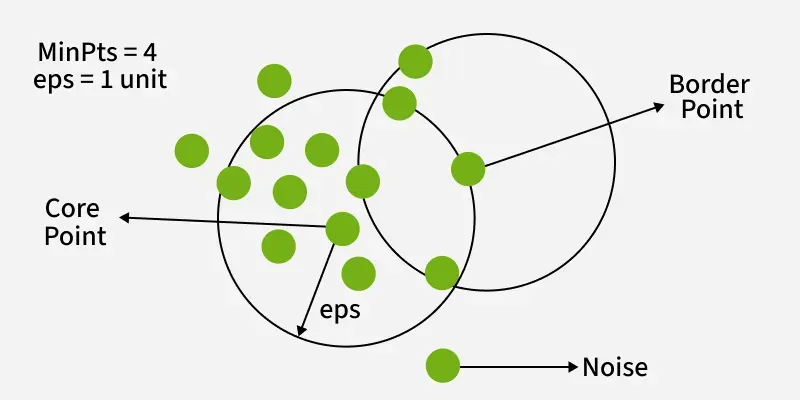
\includegraphics[width=0.95\linewidth,height=0.62\textheight,keepaspectratio]{images/dbscan-core-border-noise.png}
      \end{center}
    \end{column}
  \end{columns}
\end{frame}

% Slide 16: DBSCAN & OPTICS - Formula Intuition
\begin{frame}{DBSCAN \& OPTICS: Mathematical Rationale \& Density Intuition}
  \small
  \begin{columns}[T]
    \begin{column}{0.5\textwidth}
      \textbf{1. Intuition of Density Thresholding:}
      \begin{itemize}\setlength{\itemsep}{1.5pt}
        \item Neighborhood ball: $N_\varepsilon(p) = \{q \in \mathcal{X} \mid d(p, q) \le \varepsilon\}$.
        \item \textbf{Local density threshold is defined as:}
          $$\rho_{\min} = \frac{\text{MinPts}}{V_\varepsilon}, \quad V_\varepsilon \propto \varepsilon^d$$
        \item A spatial region is identified as a \textbf{"Cluster"} if and only if empirical density exceeds $\rho_{\min}$.
        \item \textbf{Built-in Outlier Immunity:} Sparse points with local density $< \rho_{\min}$ are segregated immediately as Noise (Label $-1$), preserving cluster shape.
      \end{itemize}
    \end{column}
    \begin{column}{0.5\textwidth}
      \textbf{2. Intuition of Reachability Distance (OPTICS):}
      $$\text{rd}(p, o) = \max(\text{core-dist}(o), d(o, p))$$
      \begin{itemize}\setlength{\itemsep}{1.5pt}
        \item Standard DBSCAN fails when clusters have differing densities across regions.
        \item OPTICS smooths point-to-point transitions: point $p$ can only be accessed from core $o$ with at least the core-radius of $o$.
        \item \textbf{Reachability Plot:} Valleys represent high-density clusters; peaks represent cluster separators or isolated noise.
      \end{itemize}
    \end{column}
  \end{columns}
\end{frame}

% Slide 17: Hand Calculation DBSCAN
\begin{frame}{DBSCAN: Step-by-Step Hand Calculation (Core, Border, Noise)}
  \scriptsize
  \textbf{Sample Problem:} Consider 5 points in 1D: $x_1=1.0, x_2=1.8, x_3=2.5, x_4=5.0, x_5=9.0$.\\
  \textbf{Hyperparameters:} Neighborhood radius $\varepsilon = 1.0$, Minimum points $\text{MinPts} = 2$.
  
  \vspace{0.4em}
  \begin{columns}[T]
    \begin{column}{0.52\textwidth}
      \textbf{Step 1: Scan $\varepsilon$-Neighborhood for Each Point}
      \begin{itemize}\setlength{\itemsep}{1.5pt}
        \item Point $x_1(1.0)$: $N_{1.0}(x_1) = \{x_1, x_2\}$ since $|1.0-1.8| = 0.8 \le 1.0$.
          Neighbor count $= \mathbf{2 \ge \text{MinPts}} \implies \mathbf{Core\ Point}$.
        \item Point $x_2(1.8)$: $N_{1.0}(x_2) = \{x_1, x_2, x_3\}$ since $|1.8-1.0|=0.8, |1.8-2.5|=0.7$.
          Neighbor count $= \mathbf{3 \ge \text{MinPts}} \implies \mathbf{Core\ Point}$.
        \item Point $x_3(2.5)$: $N_{1.0}(x_3) = \{x_2, x_3\}$ since $|2.5-1.8| = 0.7 \le 1.0$.
          Neighbor count $= \mathbf{2 \ge \text{MinPts}} \implies \mathbf{Core\ Point}$.
        \item Point $x_4(5.0)$: $N_{1.0}(x_4) = \{x_4\}$ (only itself).
          Neighbor count $= \mathbf{1 < \text{MinPts}}$ and nearest Core $x_3$ is $2.5 > \varepsilon \implies \mathbf{Noise\ Point}$.
        \item Point $x_5(9.0)$: $N_{1.0}(x_5) = \{x_5\}$.
          Neighbor count $= \mathbf{1 < \text{MinPts}} \implies \mathbf{Noise\ Point}$.
      \end{itemize}
    \end{column}
    \begin{column}{0.48\textwidth}
      \textbf{Step 2: Density-Connected Cluster Expansion}
      \begin{itemize}\setlength{\itemsep}{2pt}
        \item Seed from Core $x_1$: annexes $x_2$.
        \item From Core $x_2$: annexes $x_3$.
        \item Points $x_1, x_2, x_3$ form a single density-connected cluster!
      \end{itemize}
      \vspace{0.2em}
      \textbf{Complete Partition Summary:}
      \begin{table}[]
        \centering
        \begin{tabular}{c c l}
          \toprule
          \textbf{Point} & \textbf{Topological Role} & \textbf{Cluster Label} \\
          \midrule
          $x_1, x_2, x_3$ & Core Point & \textbf{Cluster 1} \\
          $x_4$ & Noise & \textbf{Outlier (Label -1)} \\
          $x_5$ & Noise & \textbf{Outlier (Label -1)} \\
          \bottomrule
        \end{tabular}
      \end{table}
      \textbf{Takeaway:} DBSCAN seamlessly extracts non-trivial dense structures while isolating anomalous points $x_4, x_5$!
    \end{column}
  \end{columns}
\end{frame}

% Slide 18: Density-based - Applications & Suitability
\begin{frame}{Density-based: Real-World Applications \& Suitability Guide}
  \footnotesize
  \begin{columns}[T]
    \begin{column}{0.5\textwidth}
      \textbf{1. Practical Applications:}
      \begin{itemize}\setlength{\itemsep}{2pt}
        \item \textbf{Credit Card Fraud \& Network Intrusion Detection:}
          Legitimate transactions form dense behavioral clusters. Fraudulent wash-trading or DDoS attacks lie isolated in sparse density voids $\to$ DBSCAN automatically flags them as Noise ($-1$).
        \item \textbf{GPS Fleet Telematics \& Smart Urban Transit (Uber, Grab):}
          Clusters millions of pickup/drop-off GPS coordinates to extract urban traffic bottlenecks and passenger hotspots without distortion from GPS signal drift.
        \item \textbf{Astronomy \& Cosmology:}
          Extracts stellar streams and spiral galaxy arms against vast cosmic vacuum noise.
      \end{itemize}
    \end{column}
    \begin{column}{0.5\textwidth}
      \textbf{2. When to Use vs When NOT to Use:}
      \begin{itemize}\setlength{\itemsep}{2pt}
        \item \textcolor{darkgreen}{\textbf{RECOMMENDED WHEN:}}
          \begin{itemize}
            \item Clusters exhibit arbitrary, non-linear, non-spherical shapes (concentric rings, crescents).
            \item High ratio of noise and anomalies requiring automated filtration.
            \item The number of clusters $K$ cannot be known in advance.
          \end{itemize}
        \item \textcolor{crimsonred}{\textbf{AVOID WHEN:}}
          \begin{itemize}
            \item Clusters have large density variations (upgrade to \textbf{OPTICS} or \textbf{HDBSCAN}).
            \item Very high feature dimensions ($d > 20$) where distance concentration makes fixed $\varepsilon$ spheres ineffective (Curse of Dimensionality).
          \end{itemize}
      \end{itemize}
    \end{column}
  \end{columns}
\end{frame}

% Slide 19: Distribution-based - GMM & EM
\begin{frame}{5. Distribution-based: Gaussian Mixture Models (GMM)}
  \begin{columns}[T]
    \begin{column}{0.55\textwidth}
      \textbf{Generative Probabilistic Model:}
      $$p(x) = \sum_{k=1}^K \pi_k \mathcal{N}(x \mid \mu_k, \Sigma_k)$$
      \begin{itemize}\setlength{\itemsep}{1pt}
        \item $\pi_k$: Component mixing weight ($\sum \pi_k = 1, \pi_k \ge 0$).
        \item $\mu_k$: Mean vector (cluster centroid).
        \item $\Sigma_k$: Covariance matrix (ellipsoidal geometry/orientation).
      \end{itemize}
      \textbf{Soft Membership (Posterior Responsibility):}
      $$\gamma_{nk} = P(z_{nk}=1 \mid x_n) = \frac{\pi_k \mathcal{N}(x_n \mid \mu_k, \Sigma_k)}{\sum_{j=1}^K \pi_j \mathcal{N}(x_n \mid \mu_j, \Sigma_j)}$$
    \end{column}
    \begin{column}{0.45\textwidth}
      \begin{center}
        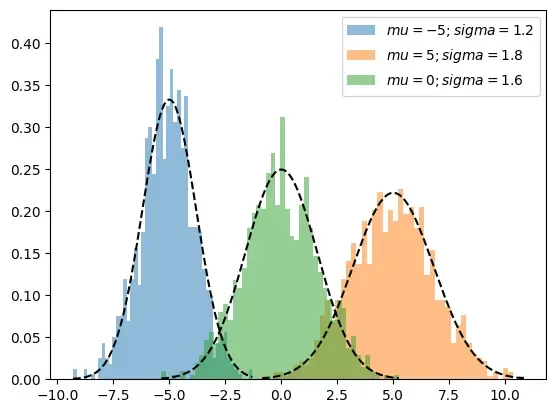
\includegraphics[width=0.92\linewidth,height=0.62\textheight,keepaspectratio]{images/gmm-distribution-concept.png}
      \end{center}
    \end{column}
  \end{columns}
\end{frame}

% Slide 20: EM Algorithm - Formula Intuition
\begin{frame}{EM Algorithm: Mathematical Rationale \& E-step / M-step Intuition}
  \small
  \begin{columns}[T]
    \begin{column}{0.5\textwidth}
      \textbf{1. Intuition of the E-step (Expectation):}
      $$\gamma_{nk} = \frac{\pi_k \mathcal{N}(x_n \mid \mu_k, \Sigma_k)}{\sum_{j=1}^K \pi_j \mathcal{N}(x_n \mid \mu_j, \Sigma_j)}$$
      \begin{itemize}\setlength{\itemsep}{1.5pt}
        \item Direct application of \textbf{Bayes' Theorem}: Evaluates the posterior probability that sample $x_n$ was generated by component $k$.
        \item Replaces rigid binary assignments with \textbf{"soft responsibility"} fractions (e.g., $85\%$ Cluster 1, $15\%$ Cluster 2).
      \end{itemize}
    \end{column}
    \begin{column}{0.5\textwidth}
      \textbf{2. Intuition of the M-step (Maximization):}
      $$\mu_k = \frac{\sum_{n=1}^N \gamma_{nk} x_n}{\sum_{n=1}^N \gamma_{nk}}, \quad N_k = \sum_{n=1}^N \gamma_{nk}$$
      $$\Sigma_k = \frac{1}{N_k}\sum_{n=1}^N \gamma_{nk} (x_n - \mu_k)(x_n - \mu_k)^T$$
      \begin{itemize}\setlength{\itemsep}{1.5pt}
        \item Every data point contributes to adjusting centroid $\mu_k$ and shape $\Sigma_k$ weighted exactly by its responsibility $\gamma_{nk}$.
        \item \textbf{Mathematical Guarantee:} Incomplete log-likelihood $\ln p(\mathcal{X} \mid \theta)$ monotonically increases at every EM iteration!
      \end{itemize}
    \end{column}
  \end{columns}
\end{frame}

% Slide 21: Hand Calculation GMM E-step
\begin{frame}{GMM: Step-by-Step Hand Calculation (E-step Responsibility $\gamma$)}
  \scriptsize
  \textbf{Sample Problem:} Consider 2 Gaussian components in 1D: Component 1 $\sim \mathcal{N}(\mu_1=2.0, \sigma_1^2=1.0)$, Component 2 $\sim \mathcal{N}(\mu_2=6.0, \sigma_2^2=1.0)$.\\
  Equal prior mixture weights: $\pi_1 = \pi_2 = 0.5$. Calculate soft responsibility $\gamma_1, \gamma_2$ for observation $x = 3.0$.
  
  \vspace{0.4em}
  \begin{columns}[T]
    \begin{column}{0.52\textwidth}
      \textbf{Step 1: Compute Gaussian Density Values $\mathcal{N}(x \mid \mu, \sigma)$}
      1D Gaussian PDF: $\mathcal{N}(x \mid \mu, \sigma) = \frac{1}{\sigma \sqrt{2\pi}} e^{-\frac{(x - \mu)^2}{2\sigma^2}}$.
      With $\sigma=1.0 \implies \frac{1}{\sqrt{2\pi}} \approx 0.3989$.
      \begin{itemize}\setlength{\itemsep}{2pt}
        \item Component 1: $\mathcal{N}_1(3 \mid 2, 1) = 0.3989 \cdot e^{-0.5} \approx \mathbf{0.2420}$
        \item Component 2: $\mathcal{N}_2(3 \mid 6, 1) = 0.3989 \cdot e^{-4.5} \approx \mathbf{0.0044}$
      \end{itemize}
    \end{column}
    \begin{column}{0.48\textwidth}
      \textbf{Step 2: Compute Posterior Responsibilities (E-step)}
      Total marginal density:
      $$p(x=3) = 0.5(0.2420) + 0.5(0.0044) = \mathbf{0.1232}$$
      
      Applying Bayes' Rule for responsibilities $\gamma$:
      $$\gamma_1 = \frac{0.5 \times 0.2420}{0.1232} = \frac{0.1210}{0.1232} \approx \mathbf{0.982\ (98.2\%)}$$
      $$\gamma_2 = \frac{0.5 \times 0.0044}{0.1232} = \frac{0.0022}{0.1232} \approx \mathbf{0.018\ (1.8\%)}$$
      
      \textbf{Interpretation:} Observation $x=3.0$ belongs to Component 1 with $98.2\%$ posterior certainty and to Component 2 with $1.8\%$.
    \end{column}
  \end{columns}
\end{frame}

% Slide 22: Distribution-based - Applications & Suitability
\begin{frame}{Distribution-based: Real-World Applications \& Suitability Guide}
  \small
  \begin{columns}[T]
    \begin{column}{0.5\textwidth}
      \textbf{1. Practical Applications:}
      \begin{itemize}\setlength{\itemsep}{2pt}
        \item \textbf{Speech Processing \& Speaker Diarization:}
          Automatically determines "who spoke when" in conference recordings by modeling speaker MFCC acoustic feature vectors as a mixture of Gaussians.
        \item \textbf{Brain MRI Image Segmentation:}
          Soft tissue boundaries exhibit partial volume effects across gray matter, white matter, and cerebrospinal fluid. GMM's soft membership realistically captures continuous tissue mixtures.
        \item \textbf{Quantitative Finance \& Regime Switching:}
          Models asset returns exhibiting multimodal distributions (Bull, Bear, and Stagnant regimes).
      \end{itemize}
    \end{column}
    \begin{column}{0.5\textwidth}
      \textbf{2. When to Use vs When NOT to Use:}
      \begin{itemize}\setlength{\itemsep}{2pt}
        \item \textcolor{darkgreen}{\textbf{RECOMMENDED WHEN:}}
          \begin{itemize}
            \item Clusters have oriented ellipsoidal shapes with diverse sizes and covariances.
            \item Business problem requires soft probabilities to quantify decision uncertainty.
            \item Clusters naturally overlap along realistic boundaries.
          \end{itemize}
        \item \textcolor{crimsonred}{\textbf{AVOID WHEN:}}
          \begin{itemize}
            \item Clusters are non-ellipsoidal (crescents, rings).
            \item High dimensionality causes full covariance matrices $\Sigma_k$ ($d \times d$) to overfit or become singular.
          \end{itemize}
      \end{itemize}
    \end{column}
  \end{columns}
\end{frame}

% Slide 23: Fuzzy Clustering - Fuzzy C-Means (FCM)
\begin{frame}{Paradigm 5: Fuzzy Clustering (Fuzzy C-Means - FCM)}
  \small
  \begin{columns}[T]
    \begin{column}{0.55\textwidth}
      \textbf{Essence of Fuzzy Clustering (Bezdek, 1981):}
      \begin{itemize}\setlength{\itemsep}{1pt}
        \item Soft generalization of K-Means where each point belongs to all clusters with fuzzy degree $u_{ik} \in [0, 1]$ satisfying $\sum_{k=1}^K u_{ik} = 1$.
      \end{itemize}
      \textbf{Fuzzy Objective ($m > 1$ is the fuzzifier):}
      $$J_m = \sum_{i=1}^N \sum_{k=1}^K u_{ik}^m \|x_i - \mu_k\|^2 \to \min$$
      \textbf{Iterative Update Rules:}
      $$u_{ik} = \frac{1}{\sum_{j=1}^K \left(\frac{\|x_i - \mu_k\|}{\|x_i - \mu_j\|}\right)^{\frac{2}{m-1}}}, \quad \mu_k = \frac{\sum_{i=1}^N u_{ik}^m x_i}{\sum_{i=1}^N u_{ik}^m}$$
    \end{column}
    \begin{column}{0.45\textwidth}
      \textbf{Step-by-Step Hand Calculation ($m=2$):}
      \begin{itemize}\setlength{\itemsep}{1.5pt}\scriptsize
        \item Point $x=2.0$ between centroids $\mu_1=1.0, \mu_2=5.0$.
        \item Distances: $d_1 = |2-1|=1.0$, $d_2 = |2-5|=3.0$.
        \item Membership in Cluster 1:
          $$u_1 = \frac{1}{\left(\frac{1}{1}\right)^2 + \left(\frac{1}{3}\right)^2} = \frac{1}{1 + \frac{1}{9}} = \mathbf{0.9\ (90\%)}$$
        \item Membership in Cluster 2: $u_2 = 1 - 0.9 = \mathbf{0.1\ (10\%)}$.
      \end{itemize}
      \vspace{0.3em}
      \textbf{Applications \& Suitability:}
      Omnichannel customer profiling and histopathology boundary delineation without imposing Gaussian parametric assumptions.
    \end{column}
  \end{columns}
\end{frame}

% Slide 24: Model Evaluation
\begin{frame}{6. Clustering Quality Evaluation: Metric Rationale}
  \footnotesize
  \begin{columns}[T]
    \begin{column}{0.52\textwidth}
      \textbf{Deconstructing the Silhouette Coefficient ($s \in [-1, 1]$):}
      $$s(i) = \frac{b(i) - a(i)}{\max(a(i), b(i))}$$
      \begin{itemize}\setlength{\itemsep}{1.5pt}
        \item $\mathbf{a(i)}$: Mean intra-cluster distance from $i$ to all peers in the same cluster (\textbf{Cohesion}). Smaller is better!
        \item $\mathbf{b(i)}$: Mean distance from $i$ to points in the nearest neighbor cluster (\textbf{Separation}). Larger is better!
        \item \textbf{Value Interpretation:}
          \begin{itemize}
            \item $s \approx +1$: $b(i) \gg a(i) \implies$ Point is dense and far from neighboring clusters.
            \item $s \approx 0$: $a(i) \approx b(i) \implies$ Point lies directly on decision boundary.
            \item $s < 0$: $a(i) > b(i) \implies$ Point is erroneously assigned!
          \end{itemize}
      \end{itemize}
    \end{column}
    \begin{column}{0.48\textwidth}
      \textbf{Internal Validation Indices:}
      \begin{itemize}\setlength{\itemsep}{2pt}
        \item \textbf{Davies-Bouldin Index (DBI):} Ratio of intra-cluster scatter to centroid separation. \textbf{Lower is better}.
        \item \textbf{Calinski-Harabasz (CH):} Variance ratio between-cluster to within-cluster. \textbf{Higher is better}.
      \end{itemize}
      \vspace{0.3em}
      \textbf{External Validation Indices (Ground Truth Available):}
      \begin{itemize}\setlength{\itemsep}{1.5pt}
        \item \textbf{Adjusted Rand Index (ARI $\in [-1, 1]$):} Chance-adjusted pairwise cluster agreement.
        \item \textbf{NMI ($[0, 1]$):} Normalized Mutual Information.
      \end{itemize}
    \end{column}
  \end{columns}
\end{frame}

% Slide 25: Comparison Table
\begin{frame}{Comprehensive Comparison Across 5 Clustering Paradigms}
  \begin{table}[]
    \tiny
    \centering
    \begin{tabularx}{\textwidth}{l *{5}{>{\raggedright\arraybackslash}X}}
      \toprule
      \textbf{Criterion} & \textbf{K-Means} & \textbf{Hierarchical} & \textbf{DBSCAN} & \textbf{OPTICS} & \textbf{GMM / FCM} \\
      \midrule
      \textbf{Assignment Type} & Hard & Hard & Hard & Hard & \textbf{Soft (Probabilistic)} \\
      \textbf{Pre-specify $K$?} & \textbf{Required} & No & No & No & \textbf{Required} \\
      \textbf{Cluster Geometry} & Convex spherical & Spherical / Flexible & \textbf{Arbitrary (Non-linear)} & \textbf{Arbitrary (Non-linear)} & \textbf{Oriented Ellipsoids} \\
      \textbf{Multi-density} & Poor & Moderate & Poor & \textbf{Excellent} & Good \\
      \textbf{Outlier Handling} & Sensitive (Centroid pull) & Poor & \textbf{Automated Filter} & \textbf{Automated Filter} & Moderate \\
      \textbf{Time Complexity} & $O(N \cdot K \cdot I)$ & $O(N^2 \log N)$ & $O(N \log N) \to O(N^2)$ & $O(N \log N) \to O(N^2)$ & $O(N \cdot K \cdot I \cdot d^3)$ \\
      \textbf{Space Complexity} & $O(N \cdot d)$ & $O(N^2)$ & $O(N)$ & $O(N)$ & $O(N \cdot d + K \cdot d^2)$ \\
      \textbf{Visual Output} & Centroids, Voronoi & Dendrogram & Discrete Labels & Reachability Plot & Confidence Ellipses \\
      \bottomrule
    \end{tabularx}
  \end{table}
\end{frame}

% Slide 26: Decision Tree
\begin{frame}{Practical Decision Tree for Algorithm Selection}
  \begin{center}
    \resizebox{0.90\textwidth}{!}{
    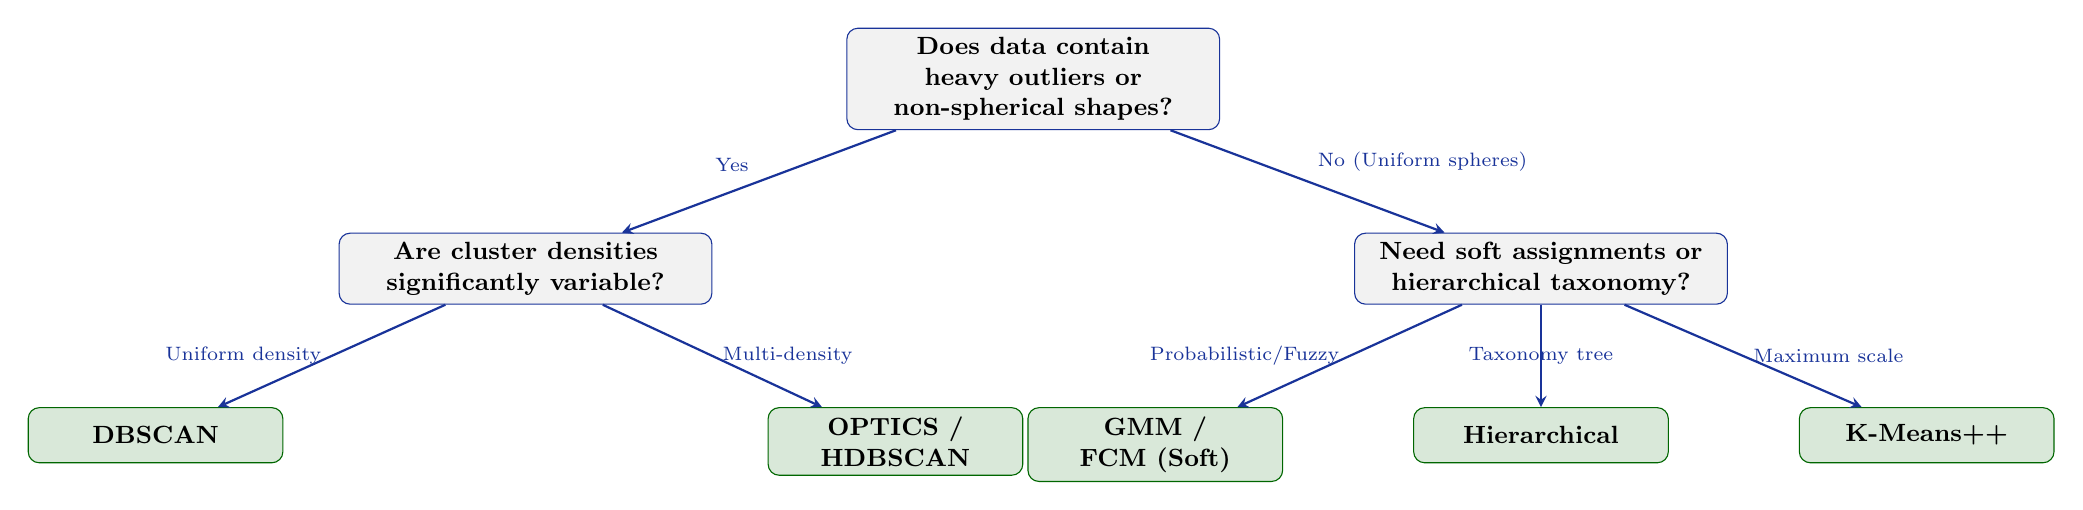
\begin{tikzpicture}[
      node distance=1.3cm and 1.2cm,
      box/.style={rectangle, draw=codeblue, fill=codegray, text centered, rounded corners, font=\small\bfseries, minimum height=0.8cm, text width=4.5cm},
      leaf/.style={rectangle, draw=darkgreen, fill=darkgreen!15, text centered, rounded corners, font=\small\bfseries, minimum height=0.7cm, text width=3.0cm},
      arrow/.style={->, >=stealth, thick, color=codeblue}
    ]
      \node[box] (root) {Does data contain heavy outliers or non-spherical shapes?};
      
      \node[box, below left=of root, xshift=-0.5cm] (density) {Are cluster densities significantly variable?};
      \node[box, below right=of root, xshift=0.5cm] (normal) {Need soft assignments or hierarchical taxonomy?};
      
      \node[leaf, below left=of density, xshift=0.5cm] (dbscan) {DBSCAN};
      \node[leaf, below right=of density, xshift=-0.5cm] (optics) {OPTICS / HDBSCAN};
      
      \node[leaf, below left=of normal, xshift=0.3cm] (gmm) {GMM / FCM (Soft)};
      \node[leaf, below=of normal] (hier) {Hierarchical};
      \node[leaf, below right=of normal, xshift=-0.3cm] (kmeans) {K-Means++};
      
      \draw[arrow] (root) -- node[above left, font=\scriptsize]{Yes} (density);
      \draw[arrow] (root) -- node[above right, font=\scriptsize]{No (Uniform spheres)} (normal);
      
      \draw[arrow] (density) -- node[left, font=\scriptsize]{Uniform density} (dbscan);
      \draw[arrow] (density) -- node[right, font=\scriptsize]{Multi-density} (optics);
      
      \draw[arrow] (normal) -- node[left, font=\scriptsize]{Probabilistic/Fuzzy} (gmm);
      \draw[arrow] (normal) -- node[font=\scriptsize]{Taxonomy tree} (hier);
      \draw[arrow] (normal) -- node[right, font=\scriptsize]{Maximum scale} (kmeans);
    \end{tikzpicture}
    }
  \end{center}
\end{frame}

% Slide 27: Scenario Suitability Matrix
\begin{frame}{Scenario Suitability Matrix: When to Use Which Algorithm?}
  \begin{table}[]
    \tiny
    \centering
    \begin{tabularx}{\textwidth}{p{3.2cm} p{2.4cm} X}
      \toprule
      \textbf{Application \& Data Profile} & \textbf{Recommended Algorithm} & \textbf{Technical Rationale \& Key Considerations} \\
      \midrule
      \textbf{E-commerce Customer Segmentation} ($N > 10^6$, continuous RFM) & \textbf{K-Means++ / Mini-Batch} & Linear scalability $O(N)$, interpretable centroids for executive marketing campaigns. \\
      \addlinespace
      \textbf{Anti-Money Laundering \& Fraud} (Substantial noise and outliers) & \textbf{DBSCAN} & Automatically segregates anomalous transactions into Noise ($-1$) without corrupting clusters. \\
      \addlinespace
      \textbf{GPS Urban Fleet Routing} (Multi-density transit corridors) & \textbf{OPTICS / HDBSCAN} & Traces non-linear arterial roads across diverse traffic density levels. \\
      \addlinespace
      \textbf{Retail Category Taxonomy, Gene Microarrays} ($N < 5{,}000$) & \textbf{Hierarchical (Ward Linkage)} & Dendrogram provides an interpretable multi-level tree without guessing $K$ in advance. \\
      \addlinespace
      \textbf{Brain MRI Tissue Segmentation, Meeting Speaker Diarization} & \textbf{GMM (EM Algorithm)} & Soft posterior probabilities quantify partial volume ambiguity across overlapping boundaries. \\
      \addlinespace
      \textbf{Borderline Credit Scoring, Omnichannel Customer Profiles} & \textbf{Fuzzy C-Means (FCM)} & Continuous membership degrees $u_{ik} \in [0, 1]$ model ambivalent cross-category consumer behavior. \\
      \bottomrule
    \end{tabularx}
  \end{table}
\end{frame}

% Slide 28: Challenges & Limitations
\begin{frame}{Core Challenges \& Limitations in Clustering}
  \small
  \begin{columns}[T]
    \begin{column}{0.5\textwidth}
      \textbf{1. Determining Optimal Cluster Count $K$:}
      \begin{itemize}\setlength{\itemsep}{2pt}
        \item In the absence of labels, selecting $K$ is fundamentally heuristic.
        \item Requires triangulation across Elbow, Silhouette, DBI, and domain business requirements.
      \end{itemize}
      \vspace{0.4em}
      \textbf{2. Sensitivity to Initialization \& Outliers:}
      \begin{itemize}\setlength{\itemsep}{2pt}
        \item Random seed initialization risks trap in severe local minima (mitigated by K-Means++).
        \item Outliers exert extreme leverage on arithmetic centroids.
      \end{itemize}
    \end{column}
    \begin{column}{0.5\textwidth}
      \textbf{3. Curse of Dimensionality:}
      \begin{itemize}\setlength{\itemsep}{2pt}
        \item As dimension $d$ grows, pairwise distances converge toward uniform values (Distance Concentration).
        \item \textit{Solution:} Mandatory dimensionality reduction via PCA/t-SNE/UMAP before clustering.
      \end{itemize}
      \vspace{0.4em}
      \textbf{4. Computational Limits on Big Data:}
      \begin{itemize}\setlength{\itemsep}{2pt}
        \item Hierarchical ($O(N^2)$ memory) fails on $N > 20{,}000$.
        \item Must transition to Mini-Batch K-Means, BIRCH, or scalable approximations.
      \end{itemize}
    \end{column}
  \end{columns}
\end{frame}

% Slide 29: Summary & Lab Roadmap
\begin{frame}{Summary \& Hands-on Lab Roadmap}
  \begin{columns}[T]
    \begin{column}{0.5\textwidth}
      \textbf{Lecture Key Takeaways:}
      \begin{itemize}\setlength{\itemsep}{2pt}
        \item Clustering is data science's most potent lens for uncovering latent natural structure.
        \item \textit{No Free Lunch Theorem:} No single clustering algorithm universally outperforms across all datasets.
        \item Algorithm selection strictly depends on:
          \begin{itemize}\setlength{\itemsep}{1pt}
            \item Dataset scale $N$ (Sample capacity).
            \item Cluster geometry (Convex spherical vs Non-linear).
            \item Noise ratio and outlier prevalence.
            \item Business assignment mode (Hard vs Soft).
          \end{itemize}
      \end{itemize}
    \end{column}
    \begin{column}{0.5\textwidth}
      \textbf{Laboratory Practicum in Python Notebook:}
      \begin{enumerate}\setlength{\itemsep}{2pt}
        \item \textbf{Step-by-Step Hand Calculations:}
          \begin{itemize}
            \item 1 iteration of K-Means on toy coordinates.
            \item Agglomerative Single/Complete Linkage merge.
            \item Core/Border/Noise classification in DBSCAN.
            \item 1 cycle of E-step \& M-step in GMM.
          \end{itemize}
        \item \textbf{Guided Fill-in-the-Blank Coding Labs:}
          \begin{itemize}
            \item Scikit-Learn \& SciPy implementation.
            \item Automated assert testing and validation.
          \end{itemize}
      \end{enumerate}
    \end{column}
  \end{columns}
\end{frame}

\end{document}
